\section{Theorie}
\label{sec:Theorie}

\subsection{Interferenz von elektromagnetischen Wellen}
Im einfachsten Fall kann Licht als eine ebene elektromagnetische Welle dargestellt werden. Dabei hat der elektrische Feldanteil die Form
\begin{equation}
\vec{E}(x,t)=\vec{E}_.0\cdot \mathrm{e}^{i\left(kx -\omega t -\delta\right)}\label{eq:Welle},
\end{equation}
wobei $k$ die Wellenzahl und $\omega$ die Kreisfrequenz der Welle und $\delta$ eine Phasenverschiebung sind.
Aus den Maxwellgleichungen folgt, das mehrere solcher Wellen dem Superpositionsprinzip genügen und sich somit vektoriell addieren:
\[
\vec{E}=\vec{E}_.1+\vec{E}_.2+\text{...}
\]
Aufgrund der hohen Frequenzen der optischen Lichtwellen kann jedoch experimentell nur die Lichtintensität $I$, also der zeitliche Mittelwert der auf eine Fläche treffenden Leistung, bestimmt werden.
Es gilt:
\[
I=\frac{const}{t_.2-t_.1}\int_{t_.1}^{t_.2}|\vec{E}(x,t)|^2\mathrm{d}t
\]
und somit bei Superposition von zwei Wellen
\begin{equation}
I_.{ges}=\frac{const}{t_.2-t_.1}\int_{t_.1}^{t_.2}|\vec{E}_.1(x,t)+\vec{E}_.2(x,t)|^2\mathrm{d}t \text{.}
\end{equation}
Mit Gleichung folgt dann für die Intensität:
\begin{equation}
I_.{ges}=2\cdot const\cdot E^2_.0(1+\cos(\delta_.2-\delta_.1))
\end{equation}
Daraus lässt sich erkennen das, abhängig von der Phase der beiden Lichtwellen, die Intensität durch den Interferenzterm um bis zu $\pm 2\cdot const\cdot E^2_.0$ vom Mittelwert $2\cdot const\cdot E^2_.0$ abweichen.
Wenn gilt
\[
\delta_.2-\delta_.1=(2n+1)\pi,
\]
mit $n$ aus den natürlichen Zahlen, verschwindet die Intensität, selbst wenn die Einzelintensitäten von $0$ verschieden sind.
Dies gilt jedoch nur wenn für alle Phasenverschiebungen $\delta=const$ gilt. Wenn sie von der Zeit abhängen, führt eine zeitliche Mittelung über einen gegen die Periodendauer großen Zeitraum $t_.2-t_.1$ zum verschwinden des Interferenzterms. Das ist der Fall wenn das Licht inkoheränt ist, also wenn es nicht von derselben Lichtquelle ausgesandt wird.
\subsection{Kohärenz von Lichtwellen}
\begin{figure}
\centering
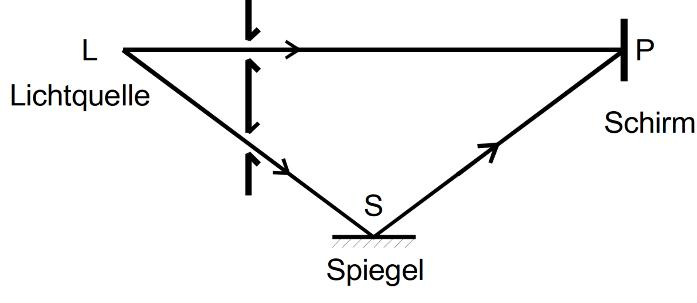
\includegraphics[scale=0.5]{content/images/kohaerenz.jpg}
\caption{Aufbau zur Erzeugung von kohärentem Licht\cite{V401}}
\label{fig:Kohärenz}
\end{figure}
\noindent Während das Licht eines Lasers immer kohärent ist, muss das einer gewöhnlichen Lichtquelle gemäß Abbildung \ref{fig:Kohärenz} durch Spiegelkonstruktionen oder Spalte aufgeteilt und umgelenkt werden, sodass es an einem Detektor durch die unterschiedlichen zurückgelegten Wegstrecken zu festen Phasenunterschieden kommt.
Da die Lichtgeschwindigkeit $c$ jedoch konstant und endlich ist, darf der Wegunterschied nicht größer werden als die Kohärenzlänge 
\[
\ell = N\lambda,
\]
mit der Wellenlänge $\lambda$ und der Anzahl $N$ der höchstens beobachtbaren Maxima der Interferenz.
Weiterhin gilt nach Fourier, dass ein Wellenpaket endlicher Länge nicht monochromatisch ist, sondern aus einem Spektrum unendlich vieler verschiedener Frequenzen zusammengesetzt ist. Zwei solcher Wellenpakete interferieren nur bedingt, da es am selben Punkt ein Minimum der einen und ein Maximum einer anderen Wellenlänge geben kann.\newline
Das Frequenzspektrum eines Wellenzuges 
\[
E(t)=\begin{cases}
E_.0\mathrm{e}^{-i\omega_.0t} & \text{für} -\frac{\tau}{2}<t<\frac{\tau}{2}\\
0 & \text{sonst}
\end{cases}
\]
der zeitlichen Länge $\tau=\ell c$ lässt sich über die Fouriertransformation berechnen:
\begin{equation*}
g(\omega)=\int_{-\inf}^{\inf}E(t)\mathrm{e}^{i\omega t}\mathrm{d}t=2E_.0\frac{sin(\frac{\tau}{2}(\omega-\omega_.0))}{\omega-\omega_.0}
\end{equation*}
Das Betragsquadrat dieser Funktion
\begin{equation*}
G(\omega)=4E^2_.0\frac{sin^2(\frac{\tau}{2}(\omega-\omega_.0))}{(\omega-\omega_.0)^2}
\end{equation*}
bezeichnet die Intensität der Schwingung für die verschiedenen Frequenzen.
$G(\omega)$ hat sein globales Maximum für $\omega =\omega_.0$. Die weiteren lokalen Maxima können vernachlässigt werden, da sie schnell gegen null streben.
Die Breite der Verteilung ist deshalb gegeben durch den Bereich um das Maximum, der von null verschieden ist und beträgt
$\Delta\omega=2\frac{\pi}{\tau}$
Die Wellenlängenverteilung dagegen hat ihr Maximum bei 
\[
\lambda_.0=\frac{2\pi c}{\omega_.0}
\]
Damit ergibt sich für die Breite der Wellenlängenverteilung
\begin{equation}
\Delta\lambda=\frac{\lambda^2_.0}{\ell}\label{eq:dl}
\end{equation}
\subsection{Brechungsindex im Medium}
Für den Brechungsindex $n$, der einer Lichtwelle im Medium widerfährt, gilt:
\begin{equation*}
n= \sqrt{1+f(\lambda)N},
\end{equation*}
mit der Anzahl $N$ der durch die Photonen angeregten Dipole pro Volumeneinheit.\newline
Für Wellenlängen im Bereich des sichtbaren Lichts gilt
\[
f(\lambda)N\ll 1,
\]
weshalb eine Taylornäherung durchgeführt werden kann und sich die Formel für $n$ zu 
\begin{equation}
n= 1+\frac{f}{2}N\label{eq:n}
\end{equation}
Im Bereich von $0$ bis $\SI{1}{\bar}$ gilt für die in diesem Experiment zu untersuchende Gase annähernd das ideale Gasgesetz:
\[
pV=Nk_.BT
\]
mit der Boltzmann-Konstanten $k_.B\approx\SI{1,38}{\joule\per\kelvin}$.
$N$ ist nun die Zahl der pro Volumeneinheit vorhandenen Teilchen und abhängig vom Druck $p$ und der Temperatur $T$ des Gases.
Unter Normalbedingungen, also einem Druck $p_.0=\SI{1,013}{\bar}$ und einer Temperatur $T_.0=\SI{273,15}{\kelvin}$ ist für 1 Mol Gas $N=N_.A\approx 6,2e23$.\newline
Allgemein gilt
\[
N(p,T)=\frac{p}{T}\frac{T_.0}{p_.0}N_.A
\]
Die Änderung des Brechungsindex bei Veränderung des Druckes von $p$ auf $p'$ und fester Temperatur $T$ erhält man mit Formel \eqref{eq:n} zu
\begin{equation}
\Delta n(p,p')=\frac{f}{2}N_.A\frac{T_.0}{p_.0}\frac{1}{T}(p-p')\label{eq:dn}
\end{equation}
Für den Brechungsindex unter Normalbedingungen gilt dann 
\begin{equation}
n(p_.0,T_.0)=1+\frac{f}{2}N_.A=1+\Delta n(p,p')\frac{T}{T_.0}\frac{p_.0}{p-p'}\text{.}\label{eq:n2}
\end{equation} 
Die Änderung des Brechungsindex $\Delta n$ kann über die Anzahl $Z$ der bei einer Druckveränderung von $p$ auf $p'$ über den Detektor wandernden Interferenzmaxima bestimmt werden.\newline Die Wellenlänge $\lambda$ des einfallenden Lichtes lässt sich über 
\begin{equation}
\lambda = 2\Delta d\cdot Z\label{eq:lambda}
\end{equation}
berechnen, wobei $\Delta d$ die Strecke bezeichnet, um die der in Strahlrichtung bewegliche Spiegel verschoben wird. Mit der Länge $b$ der Messzelle:
\begin{equation}
\Delta n = \frac{Z\lambda}{2b}
\end{equation}
Mit Gleichung \eqref{eq:n2} ergibt sich also
\begin{equation}
n(p_.0,T_.0)=1+\frac{Z\lambda}{2b}\frac{T}{T_.0}\frac{p_.0}{p-p'}\text{.}\label{eq:n3}
\end{equation}